%%%%%
% Presentación Software Libre (UJA)
% Copyright (c) 2016 Nicolás A. Ortega
% Licencia: GNU GPLv3
%%%%%
\documentclass[xetex]{beamer}
\usepackage{fontspec}
\usepackage[spanish, es-noquoting]{babel}
\usepackage{graphicx}
\DeclareGraphicsExtensions{.pdf,.png,.jpg,.jpeg}
\usepackage[export]{adjustbox}

\hypersetup{pdfstartview={Fit}} % Fit the presentation to the window by default

% Define theme
\usetheme{Copenhagen}
\usecolortheme{dove}

% Define title variables
\title{Software Libre}
\subtitle{Libertad en la Era Digital}
\author{Nicolás A. Ortega Froysa}
\institute{Universidad de Jáen}
\date{} % Keep the date blank
\subject{Software Libre}

\begin{document}
% Create the title frame
\frame{\titlepage}

%---------------------------------------------------------------

\begin{frame}
    \frametitle{Contenido}
    \tableofcontents[hideallsubsections]
\end{frame}

%---------------------------------------------------------------

\section{¿Qué es el Software Libre?}
\begin{frame}
    \centering \Huge ¿Qué es el Software Libre?
\end{frame}

%---------------------------------------------------------------

\begin{frame}
    \centering
    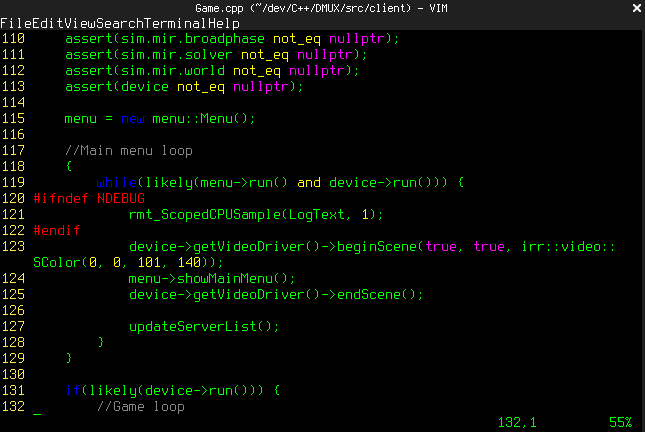
\includegraphics[scale=0.4]{imgs/source}
\end{frame}

%---------------------------------------------------------------

\begin{frame}
    \centering
    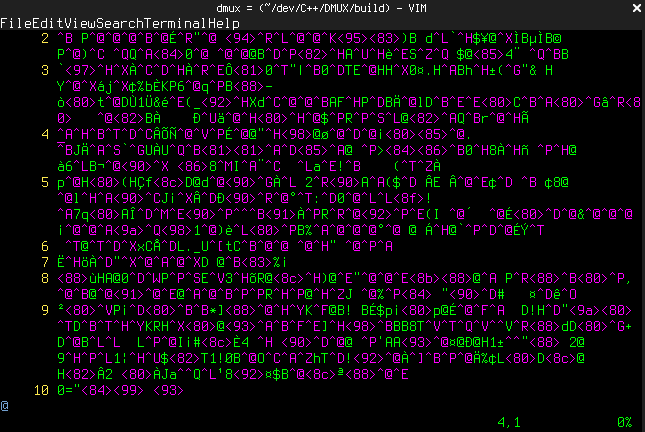
\includegraphics[scale=0.4]{imgs/binary}
\end{frame}

%---------------------------------------------------------------

\subsection{Inicios del Software Libre}
\begin{frame}
    \begin{figure}
        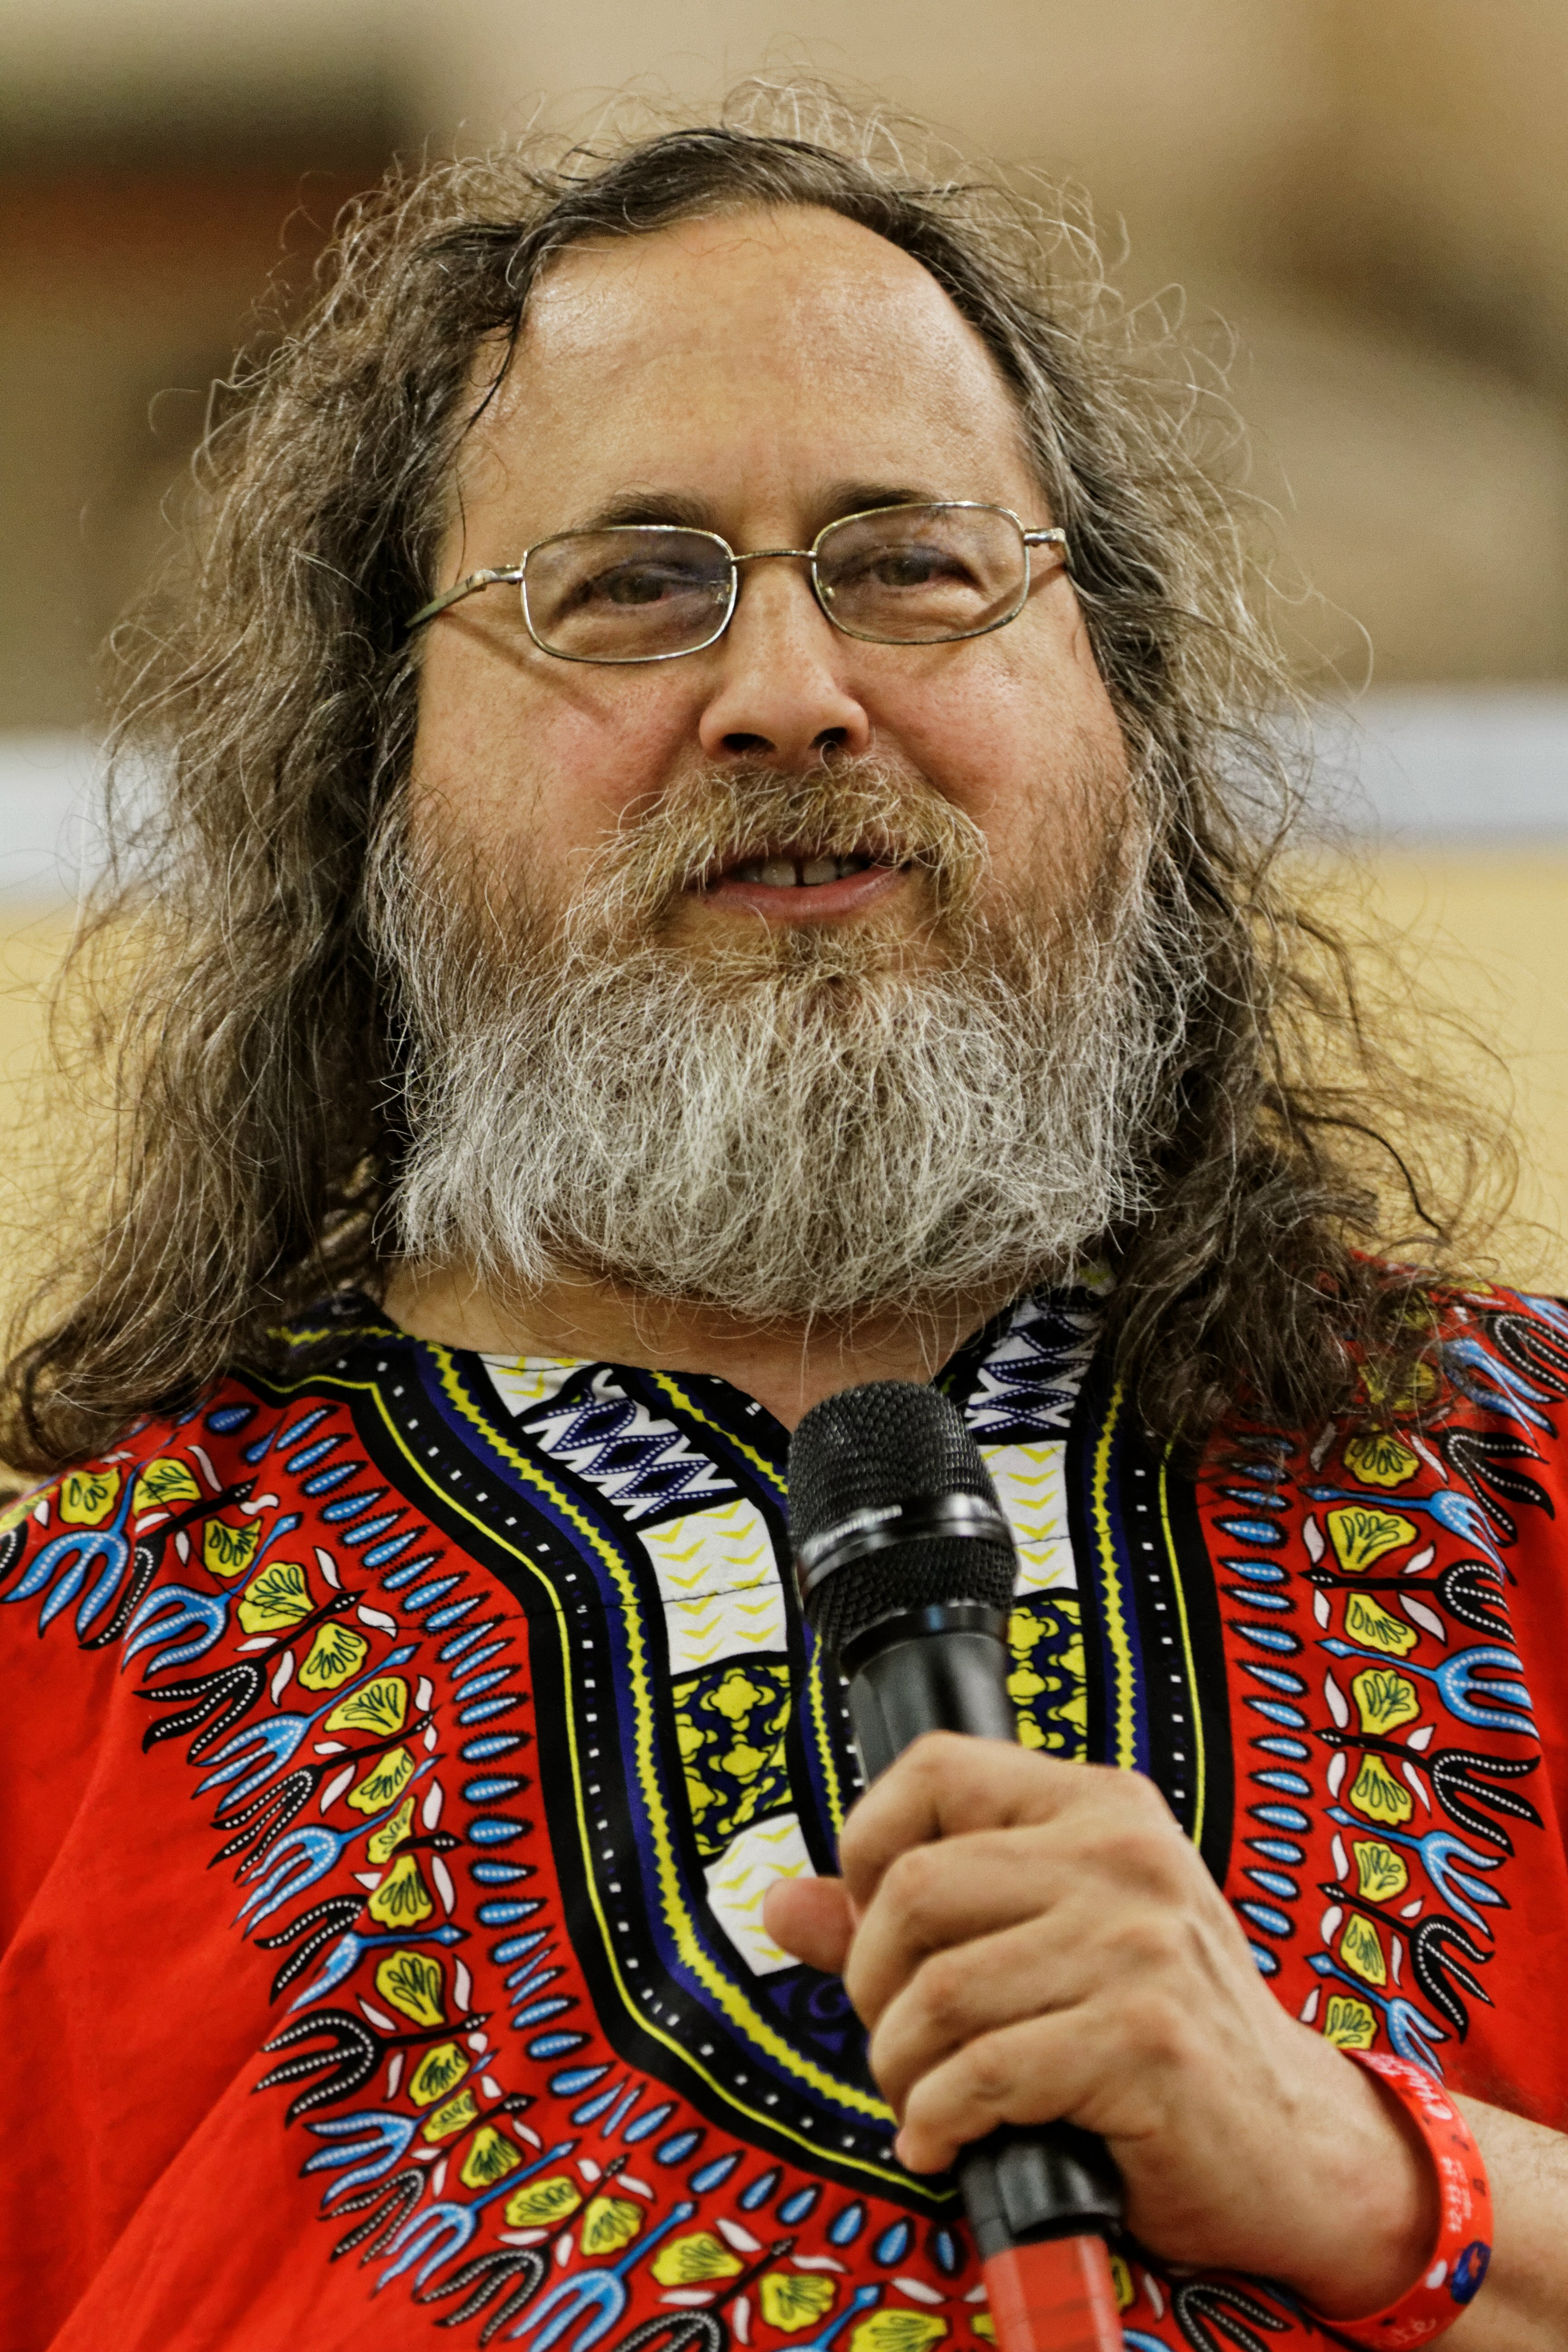
\includegraphics[width=0.35\textwidth]{imgs/rms}
        \pause{}
        \hfill
        
\includegraphics[width=0.4\textwidth]{imgs/gnuu}
    \end{figure}
    \footnotetext[1]{``Conference by Richard Stallman\ldots'', Copyright \copyright{} 2014 Thesupermat, CC-BY-SA 3.0}
    \footnotetext[2]{``gnuu~'', 4chan, N/A}
\end{frame}

%---------------------------------------------------------------

\begin{frame}
    \centering{\Large GNU\linebreak{} (GNU is Not Unix)}
    \begin{figure}
        
\includegraphics[width=0.5\textwidth]{imgs/Heckert_GNU_white}
    \end{figure}
    \footnotetext[1]{``Heckert GNU white'', Copyright \copyright{} Aurelio A. Heckert, CC-BY-SA 3.0}
\end{frame}

%---------------------------------------------------------------

\begin{frame}
    \centering{\Large FSF\linebreak{} (Free Software Foundation)}
    \begin{figure}
        
\includegraphics[width=0.5\textwidth]{imgs/fsf}
    \end{figure}
    \footnotetext[1]{``FSF logo sticker'', Copyright \copyright{} 2010 Free Software Foundation, CC-BY-SA 3.0+}
\end{frame}

%---------------------------------------------------------------

\subsection{Las Cuatro Libertades}
\begin{frame}
    \frametitle{Las Cuatro Libertades del Software Libre}
    \pause{}
    \begin{enumerate}[<+->]
        \item[0.] Ejecutar el programa como desea, con cualquier propósito.
        \item[1.] Estudiar cómo funciona el programa, y cambiarlo para que haga lo que usted quiera.
        \item[2.] Redistribuir copias para ayudar a su prójimo.
        \item[3.] Distribuir copias modificadas a terceros.
    \end{enumerate}
    \footnotetext[1]{\url{https://www.gnu.org/philosophy/free-sw.es.html}}
\end{frame}

%---------------------------------------------------------------

\subsection{Software Libre\texttt{\char32}!= Código Abierto}
\begin{frame}
    \centering \Huge \textbf{Software Libre\\!=\\Código Abierto}
\end{frame}

%---------------------------------------------------------------

\begin{frame}[t]
    \frametitle{Código Abierto pero No Software Libre}
    \pause{}
    \begin{itemize}[<+->]
        \item Unreal Engine
        \item HTML/CSS de muchas páginas web
        \item Muchos archivos de JavaScript
    \end{itemize}
\end{frame}

%---------------------------------------------------------------

\subsection{Libre\texttt{\char32}!= Gratis}
\begin{frame}
    \centering \Huge \textbf{Libre\texttt{\char32}!= Gratis}
\end{frame}

%---------------------------------------------------------------

\subsection{Ejemplos de Software Libre}
\begin{frame}
    \frametitle{Ejemplos de Software Libre}
    \pause{}
    \begin{itemize}[<+->]
        \item Mozilla Firefox
        \item Eclipse
        \item Blender
        \item Audacity
        \item Java
        \item \ldots
    \end{itemize}
\end{frame}

%---------------------------------------------------------------

\section{Software Libre en la UJA}
\begin{frame}
    \centering \Huge Software Libre en la UJA
\end{frame}

%---------------------------------------------------------------

\begin{frame}
    \frametitle{Ejemplos de Software Libre en la UJA}
    \pause{}
    \begin{itemize}[<+->]
        \item Code::Blocks
        \item MinGW
        \item Ubuntu
        \item Mozilla Firefox
        \item 8085sim
    \end{itemize}
\end{frame}

%---------------------------------------------------------------

\subsection{Importancia del Software Libre para Estudiantes}
\begin{frame}[t]
    \frametitle{Importancia del Software Libre para Estudiantes}
    \pause{}
    \begin{itemize}[<+->]
        \item Oportunidad para aprender del programa
        \item Oportunidad para contribuir a un proyecto
        \item Obtener contactos dentro del campo de la informática
        \item Acostumbrarse a trabajar en grupos
    \end{itemize}
\end{frame}

%---------------------------------------------------------------

\subsection{Importancia del Software Libre para Profesores}
\begin{frame}[t]
    \frametitle{Importancia del Software Libre para Profesores}
    \pause{}
    \begin{itemize}[<+->]
        \item Más comunidad
        \item Atención más directa a los problemas que encuentres
        \item Posibilidad de arreglar un problema y contribuir al proyecto
    \end{itemize}
\end{frame}

%---------------------------------------------------------------

\subsection{Importancia del Software Libre para la UJA}
\begin{frame}
    \frametitle{Importancia del Software Libre para la UJA}
    \pause{}
    \centering \Large Promoción y Renombre en la Informática
\end{frame}

%---------------------------------------------------------------

\subsection{Software Propietario con Alternativas Libres}
\begin{frame}
    \frametitle{Software Propietario con Alternativas Libres}
    \pause{}
    \begin{itemize}[<+->]
        \item Mathematica < SAGE, Mathics
        \item GMail < Roundcube
        \item Microsoft Office < LibreOffice, \LaTeX{}
        \item Google Drive < Hubzilla
        \item Skype < Tox, Ring, Jitsi
        \item Microsoft Windows < GNU/Linux, BSD
        \item Facebook, Twitter, LinkedIn < Diaspora*
        \item YouTube < MediaGoblin
        \item \ldots
    \end{itemize}
\end{frame}

%---------------------------------------------------------------

\section{Software Libre en el Ambito Profesional}
\begin{frame}
    \centering \Huge Software Libre en el Ámbito Profesional
\end{frame}

%---------------------------------------------------------------

\section{Buscando Alternativas}
\begin{frame}
    \frametitle{Buscando Alternativas}
    \centering \Large \url{https://prism-break.org/es/}
\end{frame}

%---------------------------------------------------------------

\section{Bibliografía}
\begin{frame}[t]
    \frametitle{Bibliografía}
    \begin{itemize}
        \item ``Free as in Freedom: Richard Stallman's Crusade for Free Software'', Copyright \copyright{} 2002 Sam Williams, GNU Free Document License
        \item \url{https://www.gnu.org/}, Sitio web de GNU
        \item \url{https://prism-break.org/es/}, PRISM Break
    \end{itemize}
\end{frame}

%---------------------------------------------------------------

\section{Licencia}
\begin{frame}
    \frametitle{Licencia}
    Copyright \copyright{} 2016 Nicolás A. Ortega
    \linebreak{}
    \linebreak{}
    Este documento está publicado bajo la licencia GNU GPLv3, y su código fuente se puede encontrar en \url{https://github.com/Deathsbreed/SoftwareLibreUJA}.
    \linebreak{}
    \linebreak{}
    Esta presentación fue posible gracias a \LaTeX, Vim, y la Universidad de Jaén.
\end{frame}

\end{document}
